\documentclass[11pt]{article}
\usepackage[utf8]{inputenc}
\usepackage[T1]{fontenc}
\usepackage{amsmath}
\usepackage{amssymb} % Needed for \eth
\usepackage{graphicx}
\usepackage{geometry}
\usepackage{tikz}
\usepackage{pgfplots} % For plots
\usepackage{ulem}     % For underline, using normalem to avoid messing with \emph
\usepackage{tcolorbox} % For boxing equations
\usepackage{braket}    % For QM state notation if needed

\geometry{a4paper, margin=1in}
\usetikzlibrary{positioning, arrows.meta, shapes.geometric} % For TikZ diagrams
\pgfplotsset{compat=1.18} % Use a recent PGFPlots version
\usetikzlibrary{calc}
% Custom commands (optional)
\newcommand{\avg}[1]{\overline{#1}}
\newcommand{\prob}[1]{P(#1)}
\newcommand{\ProbDens}[1]{\mathcal{P}(#1)} % Using script P for density
\newcommand{\vect}[1]{\vec{#1}}
\newcommand{\dd}[1]{\mathrm{d}#1} % Differential d
\newcommand{\pderiv}[2]{\frac{\partial #1}{\partial #2}}
\newcommand{\deriv}[2]{\frac{\mathrm{d} #1}{\mathrm{d} #2}}
\newcommand{\muState}{\mu\text{-state}} % Microstate
\newcommand{\OmegaE}{\Omega(E)}
\newcommand{\omegaE}{\omega(E)}
\newcommand{\PhiE}{\Phi(E)}
\newcommand{\deltaE}{\delta E}
\newcommand{\ethbar}{\text{\it{đ}}} % \eth symbol for inexact differential
\newcommand{\kb}{k_B} % Boltzmann constant
\newcommand{\gasR}{R} % Ideal gas constant
\newcommand{\partfn}{Z} % Partition function symbol
\newcommand{\grandpartfn}{\mathcal{Z}} % Grand partition function symbol

% Define a tcolorbox style for boxed equations
\tcbuselibrary{skins}
\newtcolorbox{eqbox}[1][]{
  enhanced,
  colback=yellow!10!white,
  colframe=blue!75!black,
  boxrule=1pt,
  arc=3mm,
  #1
}

\title{Physics 415 - Lecture 21: Grand Canonical Ensemble, Maximum Entropy}
\date{March 10, 2025}
\author{} % Author not specified

\begin{document}

\maketitle
\thispagestyle{empty}

\section*{Summary}

\begin{itemize}
    \item Canonical Ensemble (CE): System at fixed $T, V, N$.
    Probability of microstate $r$: $P_r = e^{-E_r/T} / \partfn = e^{-\beta E_r} / \partfn$.
    Partition function: $\partfn = \sum_r e^{-\beta E_r}$.
    Helmholtz Free Energy: $F = \avg{E} - TS = -T \ln \partfn$.
    \item Systems in "diffusive contact" (can exchange particles):
    \begin{center}
    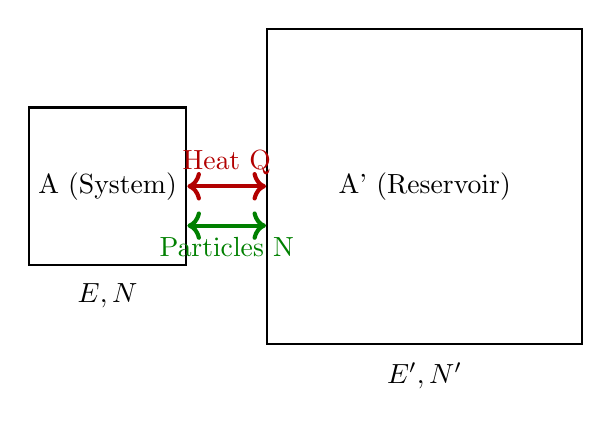
\begin{tikzpicture}
        \node (A) [draw, thick, minimum width=2cm, minimum height=2cm, label=center:A (System)] {};
        \node (Aprime) [draw, thick, minimum width=4cm, minimum height=4cm, right=1cm of A, label=center:A' (Reservoir)] {};
        \draw [line width=1.5pt, red!70!black, <->] (A.east) -- (Aprime.west) node [midway, above] {Heat Q};
        \draw [line width=1.5pt, green!50!black, <->] ($(A.east)+(0,-0.5)$) -- ($(Aprime.west)+(0,-0.5)$) node [midway, below] {Particles N};
        \node at (A.south) [below=0.1cm] {$E, N$};
        \node at (Aprime.south) [below=0.1cm] {$E', N'$};
    \end{tikzpicture}
    \end{center}
    Total system isolated: $E+E'=E^{(0)}$, $N+N'=N^{(0)}$ constant.
    Equilibrium condition: Maximize $S_{tot} = S + S'$. $dS_{tot}=0$.
    \begin{itemize}
        \item $\implies T = T'$. (Thermal Equilibrium, $1/T = (\partial S / \partial E)_{N,V}$).
        \item $\implies \mu = \mu'$. (Diffusive Equilibrium). Define Chemical Potential $\mu$:
        \[ \frac{\mu}{T} \equiv - \left( \pderiv{S}{N} \right)_{E,V} \]
        (Note: $\mu$ has energy units).
    \end{itemize}
\end{itemize}

\subsection*{Another Interpretation of $\mu$}
From $S=S(E, V, N)$, the total differential is:
\[ dS = \left(\pderiv{S}{E}\right)_{N,V} dE + \left(\pderiv{S}{V}\right)_{N,E} dV + \left(\pderiv{S}{N}\right)_{V,E} dN \]
\[ dS = \frac{1}{T} dE + \frac{p}{T} dV - \frac{\mu}{T} dN \]
Rearranging for $dE$ (Thermodynamic Identity including particle number):
\[ dE = T dS - p dV + \mu dN \]
From this, we see that $\mu$ can also be expressed as:
\[ \mu = \left( \pderiv{E}{N} \right)_{S,V} \]
Interpretation: $\mu$ is the energy cost to add one particle to the system while keeping entropy $S$ and volume $V$ fixed.
If we add $\Delta N=1$ particle: $\Delta E \approx (\partial E / \partial N)_{S,V} \times (1) = \mu$.

Similarly, consider the Helmholtz free energy $F = E - TS$, so $F=F(T, V, N)$.
$dF = dE - T dS - S dT$. Substitute $dE$:
\[ dF = (T dS - p dV + \mu dN) - T dS - S dT \]
\[ dF = -S dT - p dV + \mu dN \]
From this, we see:
\[ \mu = \left( \pderiv{F}{N} \right)_{T,V} \]
Interpretation: $\mu$ is the change in Helmholtz free energy when adding one particle at constant $T$ and $V$.

\section*{Grand Canonical Ensemble (GCE)}

Now consider the situation where system A is much smaller than reservoir A' ($|A| \ll |A'|$). A' acts as both a heat bath and a "particle reservoir" for A. The reservoir keeps the temperature $T$ and chemical potential $\mu$ of system A constant. System A can exchange both energy $E$ and particles $N$ with A'.

\begin{center}
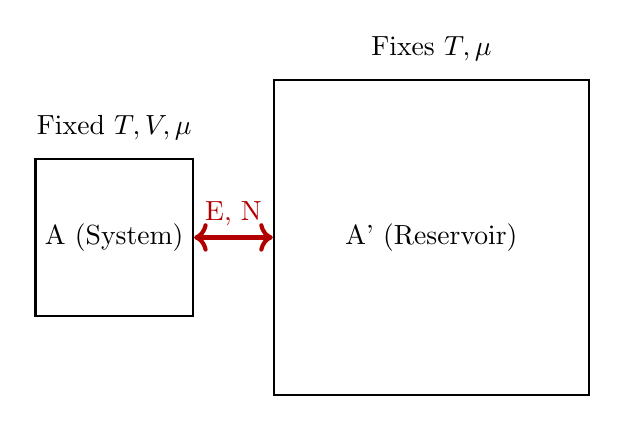
\begin{tikzpicture}
    \node (A) [draw, thick, minimum width=2cm, minimum height=2cm, label=center:A (System)] {};
    \node (Aprime) [draw, thick, minimum width=4cm, minimum height=4cm, right=1cm of A, label=center:A' (Reservoir)] {};
    \draw [line width=1.5pt, red!70!black, <->] (A.east) -- (Aprime.west) node [midway, above] {E, N};
    \node at (A.north) [above=0.1cm] {Fixed $T, V, \mu$};
    \node at (Aprime.north) [above=0.1cm] {Fixes $T, \mu$};
\end{tikzpicture}
\end{center}
Question: What is the probability distribution of microstates of A, where both $E$ and $N$ can fluctuate? (Analogous to CE where $E$ fluctuates).

Let microstate $r$ of system A have energy $E_r$ and particle number $N_r$. What is the probability $P_r$?
Proceed as for CE. $P_r$ is proportional to the number of states available to the reservoir A' when A is in state $r$. The reservoir then has energy $E' = E^{(0)} - E_r$ and particle number $N' = N^{(0)} - N_r$.
\[ P_r \propto \Omega'(E', N') = e^{S'(E', N')} \]
Since $|A| \ll |A'|$, we have $E_r \ll E^{(0)}$ and $N_r \ll N^{(0)}$. Expand $S'$ around $(E^{(0)}, N^{(0)})$:
\[ S'(E^{(0)}-E_r, N^{(0)}-N_r) \approx S'(E^{(0)}, N^{(0)}) - \left.\pderiv{S'}{E'}\right|_0 E_r - \left.\pderiv{S'}{N'}\right|_0 N_r + \dots \]
The derivatives are evaluated for the reservoir at $(E^{(0)}, N^{(0)})$, which correspond to temperature $T$ and chemical potential $\mu$.
$(\partial S'/\partial E')_0 = 1/T$.
$(\partial S'/\partial N')_0 = -\mu/T$.
\[ S'(E', N') \approx S'(E^{(0)}, N^{(0)}) - \frac{E_r}{T} - \left(-\frac{\mu}{T}\right) N_r = S'(E^{(0)}, N^{(0)}) - \frac{E_r - \mu N_r}{T} \]
Substitute back into $\Omega'$:
\[ \Omega'(E', N') \approx e^{S'(E^{(0)}, N^{(0)})} e^{-(E_r - \mu N_r)/T} = \Omega'(E^{(0)}, N^{(0)}) e^{-(E_r - \mu N_r)/T} \]
Since $P_r \propto \Omega'(E', N')$ and $\Omega'(E^{(0)}, N^{(0)})$ is a constant:
\[ P_r \propto e^{-(E_r - \mu N_r)/T} \]
Normalize the distribution: $\sum_r P_r = 1$.
Define the \textbf{Grand Partition Function} $\grandpartfn$:
\[ \grandpartfn \equiv \sum_r e^{-(E_r - \mu N_r)/T} = \sum_r e^{-\beta(E_r - \mu N_r)} \]
(Sum $r$ is over all possible states, including states with different $N_r$).
The probability distribution is:
\[ P_r = \frac{e^{-(E_r - \mu N_r)/T}}{\grandpartfn} = \frac{e^{-\beta(E_r - \mu N_r)}}{\grandpartfn} \]
This is the \textbf{Grand Canonical Distribution}.
An ensemble of systems at fixed $(T, V, \mu)$, described by this probability distribution, is the \textbf{Grand Canonical Ensemble (GCE)}.

In the GCE, both energy $E$ and particle number $N$ fluctuate. The average particle number is:
\[ \avg{N} = \sum_r P_r N_r = \frac{1}{\grandpartfn} \sum_r N_r e^{-\beta(E_r - \mu N_r)} \]
However, just as energy fluctuations are negligible in the CE for macroscopic systems, the fluctuations in particle number are also negligible in the GCE:
\[ \frac{\sqrt{\avg{\Delta N^2}}}{\avg{N}} \sim \frac{1}{\sqrt{\avg{N}}} \to 0 \quad \text{for macroscopic } \avg{N} \]
Therefore, the GCE can be used to study systems with a given (fixed) average particle number $\avg{N}$, just as the CE can be used for systems with fixed average energy $\avg{E}$.

\subsection*{Relation between $\grandpartfn$ and $Z(N)$}
It is useful to reorganize the sum over all states $r$ by first summing over states with a fixed number of particles $N$, and then summing over $N$.
Let $r \to (N, r_N)$, where $r_N$ is a state of a system with exactly $N$ particles.
$E_r \to E_{N, r_N}$ (energy of state $r_N$ with $N$ particles).
$N_r \to N$.
The grand partition function becomes:
\[ \grandpartfn = \sum_N \sum_{r_N} e^{-\beta(E_{N, r_N} - \mu N)} \]
\[ \grandpartfn = \sum_{N=0}^\infty e^{\beta \mu N} \left( \sum_{r_N} e^{-\beta E_{N, r_N}} \right) \]
The inner sum is precisely the canonical partition function $Z(T, V, N)$ for a system with a fixed number of $N$ particles:
\[ Z(T, V, N) = \sum_{r_N} e^{-\beta E_{N, r_N}} \]
Therefore, we have the relation:
\[ \grandpartfn(T, V, \mu) = \sum_{N=0}^\infty e^{\beta \mu N} Z(T, V, N) \]

\section*{Summary of Ensembles}

\begin{description}
    \item[Microcanonical (MCE):] System A isolated.
        \begin{itemize}
            \item Fixed: $E, N, V$.
            \item Prob: $P_r = 1/\Omega(E)$ (for accessible states $r$).
            \item Stat Fn: $\Omega(E) = \#$ states. $S = \ln \Omega$.
        \end{itemize}
    \item[Canonical (CE):] System A in contact with heat bath.
        \begin{itemize}
            \item Fixed: $T, N, V$. Energy $E$ fluctuates.
            \item Prob: $P_r = e^{-\beta E_r} / Z$.
            \item Stat Fn: $Z = \sum_r e^{-\beta E_r}$. $F = -T \ln Z$.
        \end{itemize}
    \item[Grand Canonical (GCE):] System A in contact with heat \& particle reservoir.
        \begin{itemize}
            \item Fixed: $T, V, \mu$. Energy $E$ and particle number $N$ fluctuate.
            \item Prob: $P_r = e^{-\beta(E_r - \mu N_r)} / \grandpartfn$.
            \item Stat Fn: $\grandpartfn = \sum_r e^{-\beta(E_r - \mu N_r)}$. Grand Potential $\Phi = -T \ln \grandpartfn$.
        \end{itemize}
\end{description}
For macroscopic systems ($N \gg 1$), all ensembles are essentially equivalent for calculating average thermodynamic properties. We choose the ensemble that is most convenient for a particular problem (usually CE or GCE, as the sums are unrestricted).
$\avg{O}_{MCE} \approx \avg{O}_{CE} \approx \avg{O}_{GCE}$.

\section*{Bonus Topic: Statistical Ensembles from Maximum Entropy}
(Ref: E.T. Jaynes, Phys. Rev. 106, 620 (1957) \& 108, 171 (1957)).
There is a unified way to think about the different statistical ensembles, based on a variational principle involving the Gibbs/Shannon entropy functional:
\[ S[\{P_r\}] = -\sum_r P_r \ln P_r \]
This entropy measures the "uncertainty" or "ignorance" represented by the probability distribution $\{P_r\}$.

\textbf{Maximum Entropy Principle:} The probability distribution $P_r$ describing our knowledge of a system is the one that maximizes $S[\{P_r\}]$ subject to the constraints imposed by the known information about the system. This yields the "least biased" distribution consistent with the given information.

\textbf{Example 1:} No information other than normalization.
Maximize $S = -\sum P_r \ln P_r$ subject to $\sum_r P_r = 1$.
Use Lagrange multiplier $\lambda$. Maximize $\tilde{S} = S - \lambda(\sum P_r - 1)$.
$\partial \tilde{S} / \partial P_r = -(\ln P_r + 1) - \lambda = 0 \implies P_r = e^{-(1+\lambda)} = \text{constant}$.
Normalization $\sum_r P_r = P \times \Omega = 1 \implies P_r = 1/\Omega$.
This recovers the Microcanonical distribution (uniform probability over accessible states $\Omega$).

\textbf{Example 2:} Known average energy $\avg{E}$.
Maximize $S$ subject to $\sum P_r = 1$ and $\sum P_r E_r = \avg{E}$.
Use two Lagrange multipliers $\lambda_1, \lambda_2$. Maximize $\tilde{S} = S - \lambda_1(\sum P_r - 1) - \lambda_2(\sum P_r E_r - \avg{E})$.
$\partial \tilde{S} / \partial P_r = -(\ln P_r + 1) - \lambda_1 - \lambda_2 E_r = 0$.
$P_r = e^{-(1+\lambda_1)} e^{-\lambda_2 E_r} = C e^{-\lambda_2 E_r}$.
Constraint $\sum P_r = 1 \implies C = 1 / (\sum_r e^{-\lambda_2 E_r})$.
\[ P_r = \frac{e^{-\lambda_2 E_r}}{\sum_r e^{-\lambda_2 E_r}} \]
This is the Canonical distribution form. The multiplier $\lambda_2$ is determined implicitly by the constraint $\sum P_r E_r = \avg{E}$. Comparing with the physical derivation of CE, we identify $\lambda_2 = \beta = 1/T$. Temperature $T$ (or $\beta$) acts as the Lagrange multiplier associated with fixing the average energy $\avg{E}$.

Similarly, one can obtain the GCE from maximizing entropy subject to known average energy $\avg{E}$ and known average particle number $\avg{N}$. The Lagrange multiplier associated with $\avg{N}$ turns out to be related to $-\beta \mu$.

\end{document}